\documentclass[12pt,fleqn]{article}
\usepackage[T1]{fontenc}
\usepackage{xiiiemc}
\usepackage{natbib}
%\usepackage{fancyhdr}
\usepackage{fancyhdr, graphicx}
\usepackage{fancyvrb}
\usepackage{color}
\usepackage{wallpaper}
\usepackage{titlesec}   %% Define space between paragraph e section
\usepackage{float} 	%% Use to fix Figure or Table: ex: \begin{table}[H]
%%%%Don't edit this block. It reduces the spacing between the lines of the
%%%%references
\let\OLDthebibliography\thebibliography
\renewcommand\thebibliography[1]{\OLDthebibliography{#1}
\setlength{\parskip}{0pt}\setlength{\itemsep}{0pt plus 0.3ex}}

%%-----------------------------------------------EDIT-----------------------------------------------
\title{Computabilidade --- Trabalho 1}

%%-----------------------------------------------EDIT----------------------------------------------
\author
    {\rm \begin{tabular}{l}
    \textbf{Ariel Nogueira Kovaljski}$^{1}$ - {\textnormal
    arielnogueirak@gmail.com}\\%
    {\fontsize{11}{0}\selectfont $^{1}$Universidade do Estado do Rio de
    Janeiro, Instituto Politécnico - Nova Friburgo, RJ,
    Brazil}\vspace*{-0.05cm} \\
  \end{tabular}}
%%----------------------------------------------------------------------------------------------
\fancypagestyle{firspagetstyle}
{

	\renewcommand{\headrulewidth}{0.0pt}
	\fancyfoot[C]{\footnotesize \parbox{15cm} {\centering
\fontsize{7.5}{0}\selectfont \it  }} % \ttfamil
	%\rhead{}
}



%%------------------

\begin{document}

\pretolerance10000
%\begin{figure}   % esse comando é para inserir a figura da logo da revista
%\centering
%
%\begin{minipage}[c]{\textwidth}
%\centering
%    
\includegraphics[width=5.75in]{logo.jpg}
%\end{minipage}
%\end{figure}

\vspace{-3cm}

\maketitle


\pagestyle{empty}

\thispagestyle{firspagetstyle}

\begin{abstract}
Este trabalho trata-se sobre a definição de programas monolíticos, iterativos e
recursivos; além disso, trata sobre a implementação de máquinas Norma e de
Turing.
\end{abstract}

\keywords{\em{Programa Monolítico, Programa Iterativo, Programa Recursivo,
Máquina Norma, Máquina de Turing}}


%---------------------------------------------------------
\fancyhead[L]{\footnotesize{\fontsize{7.5}{0}\selectfont \it}}

\renewcommand{\headrulewidth}{0.0pt}
\fancyfoot[C]{\footnotesize \parbox{15cm} {\centering
\fontsize{7.5}{0}\selectfont \it  }} % \ttfamil
\rhead{}
%---------------------------------------------------------


\pagestyle{fancy}


\section{INTRODUÇÃO}
Aqui está a introdução.

\section{DESENVOLVIMENTO}

\subsection{Definição Formal de Programas}
Um conjunto estruturado de instruções que permitem uma máquina a realização
de operações e testes sobre dados de entrada, produzindo dados de saída, pode
ser definido como um programa.

Todo programa necessita de uma estrutura de controle de operações e testes, que
permite a composição destes segundo um conjunto de regras. Dentre as linguagens
de programação atuais, os tipos de estruturação mais comuns são: monolítica,
iterativa e recursiva.

\subsubsection{Programa Monolítico}
É definido como um tipo de programa onde sua estrutura é dada apenas por
desvios condicionais e incondicionais. A sua lógica, portanto, é distribuída
por um grande bloco (monólito) que constitui o programa.

A definição formal de um programa monolítico depende dos seguintes conceitos:

\begin{enumerate}
    \item rótulo/etiqueta: palavra sobre o alfabeto de letras ou dígitos;
    \item instrução rotulada/etiquetada: cadeia de caracteres da seguinte forma
        \subitem operação --- \texttt{$r_1$: faça <$F$ | \checkmark>
        vá\_para
        $r_2$}
        \subitem \hspace{1.5em} teste --- \texttt{$r_1$: se $T$ então vá\_para
        $r_2$ senão vá\_para $r_3$}
\end{enumerate}

\noindent
Um programa monolítico $P$ é um par ordenado:
\[
    P = (I, r)
\]
onde,

\begin{enumerate}
    \item $I$: conjunto finito de instruções rotuladas, todas distintas;
    \item $r$: rótulo inicial; instrução inicial em $I$;
    \item rótulo final: caso seja referido por uma instrução de $I$, mas não
    pertença a $I$.
\end{enumerate}

É possível ilustrar um programa monolítico por meio de um fluxograma, onde cada
componente deste é representado por um bloco. Dentre os blocos disponíveis
temos o de \textit{partida}, \textit{parada}, \textit{operação} e
\textit{teste}. Um caso especial é o da operação vazia \checkmark, onde o
retângulo correspondente à operação pode ser omitido.

\begin{figure}[H]
    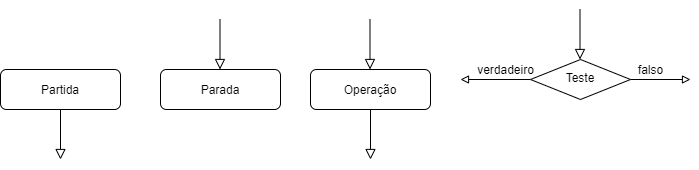
\includegraphics[width=\linewidth]{img/monolitico}
    \caption{Componentes de um programa monolítico em forma de fluxograma}
\end{figure}

\subsubsection{Exemplo de Programa Monolítico}
~ % keep title in-place

\begin{figure}[H]
\begin{verbatim}
    1: faça F vá_para 2
    2: se T1 então vá_para 1 senão vá_para 3
    3: faça G vá_para 4
    4: se T2 então vá_para 5 senão vá_para 1
\end{verbatim}
\caption{Exemplo de programa monolítico}
\end{figure}

\begin{figure}[H]
    \centering
    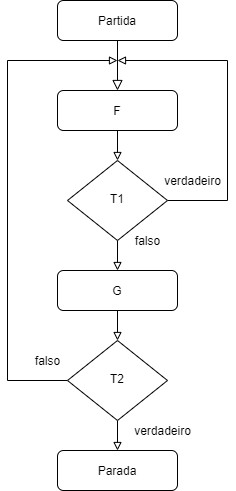
\includegraphics[height=10cm]{img/monolitico_ex}
    \caption{Exemplo de programa monolítico em forma de fluxograma}
\end{figure}

Para efeito de exemplo, considerando uma máquina de dois registradores, $(a,b)$,
as funções $F := (a := a+1) \rightarrow$ \verb|incrementa_a| e $G := (b := b-1)
\rightarrow$ \verb|decrementa_b|, os testes $T_1 := (a == 10)$ e $T_2 := (b ==
0)$ temos a seguinte máquina:

\begin{figure}[H]
\begin{verbatim}
    1: faça incrementa_a vá_para 2
    2: se (a == 10) então vá_para 1 senão vá_para 3
    3: faça decrementa_b vá_para 4
    4: se (b == 0) então vá_para 5 senão vá_para 1
\end{verbatim}
\caption{Exemplo de programa monolítico com funções e testes especificados}
\end{figure}

\noindent
Para um valor inicial de memória $(5,2)$, a computação deste programa se dá
através dos seguintes passos:

\begin{Verbatim}[commandchars=\\\{\},codes={\catcode`\$=3\catcode`\^=7}]
    (1,(5,3)) $\rightarrow$ instrução inicial e valor inicial armazenado
    (2,(6,2)) $\rightarrow$ em 1 $a$ é incrementado
    (3,(6,2)) $\rightarrow$ em 2 como $a \neq 10$, desviou para 3
    (4,(6,1)) $\rightarrow$ em 3 $b$ é decrementado
    (1,(7,1)) $\rightarrow$ em 4 como $b \neq 0$, desviou para 1
    (2,(7,1)) $\rightarrow$ em 1 $a$ é incrementado
    (3,(7,1)) $\rightarrow$ em 2 como $a \neq 10$, desviou para 3
    (4,(7,0)) $\rightarrow$ em 3 $b$ é decrementado
    (5,(7,0)) $\rightarrow$ em 4 como $b = 0$, desviou para 5. FIM.
\end{Verbatim}


\subsubsection{Programa Iterativo}
Um programa iterativo pode ser considerado uma evolução de um programa
monolítico, devido a introdução de estruturas de controle que permitem um
melhor entendimento por trás da lógica e funcionalidade do programa. Através
das estruturas de controle iterativas, evitam-se os desvios incondicionais ---
os quais tem potencial para grandes ``quebras de lógica'', como o infamo
\verb|goto| --- substituindo-os por laços de repetição. Esta prática deu origem
ao conceito de programação estruturada, a qual é utilizada pela maioria das
linguagens de programação atuais.

É possível descrever a composição de um programa iterativo como a composição de
outros programas iterativos. Sendo assim, definem-se componentes básicos aos
mesmos:

\begin{enumerate}
    \item Operação vazia \checkmark;
    \item Identificadores de operação;
    \item Composição sequencial --- \texttt{$V$;$W$}: para programas iterativos
    $V$ e $W$, esta composição resulta na execução de $V$ e, em seguida,
    execução de $W$;
    \item Composição condicional --- \texttt{(se $T$ então $V$ senão $W$)}:
    Dado uma condição de teste $T$, a composição condicional executa $V$ se $T$
    é verdadeiro ou $W$ se $T$ é falso.
    \item Composição enquanto --- \texttt{enquanto $T$ faça  ($V$)}: resulta na
    execução repetida de $V$ enquanto a condição de teste $T$ for verdadeira;
    \item Composição até --- \texttt{até $T$ faça ($V$)}: funciona de maneira
    oposta à composição enquanto; executa $V$ repetidamente enquanto $T$ for
    falso.
\end{enumerate}

\subsubsection{Exemplo de Programa Iterativo}
~ % keep title in-place



\subsubsection{Programa Recursivo}
Também encontrado na maior parte das linguagens de programação atuais, é um
tipo de estrutura onde uma rotina é composta por sub-rotinas que são compostas
de chamadas à rotina original. Desta forma, a execução de um programa recursivo
pode ser expandida em camadas, onde sucessivas chamadas à rotina em níveis cada
vez mais profundo levam a um resultado que, no fim da recursão, é
retro-propagado até a rotina de superfície.

Sub-rotinas podem ser definidas como expressões. Os seguintes itens
caracterizam-se como expressões de sub-rotinas:

\begin{enumerate}
    \item Operação vazia \checkmark;
    \item Identificadores de operação;
    \item Identificadores de sub-rotina;
    \item Composição sequencial --- \texttt{($D_1$;$D_2$)}: Para $D_1$ e $D_2$
    expressões de sub-rotinas, a sua composição sequencial resulta na execução
    de $D_1$ e, em seguida, execução de $D_2$;
    \item Composição condicional --- \texttt{(se $T$ então $D_1$ senão $D_2$)}:
    Dado um condição de teste $T$, a composição condicional é uma expressão de
    sub-rotinas que executa $D_1$ se $T$ é verdadeiro ou $D_2$ se $T$ é falso.
\end{enumerate}

Um programa recursivo $P$, portanto, pode ser definido por uma composição de
expressões de sub-rotinas, de forma que:
\[
    P \text{\tt\ é\ } E_0 \text{\tt\ onde\ } R_1 \text{\tt\ def\ } E_1, R_2
    \text{\tt\ def\ } E_2, \dots, R_n \text{\tt\ def\ } E_n
\]

Para cada $E_k, k \in \{1, 2, \dots, n\}$, temos:

\begin{itemize}
    \item $E_0$: Expressão inicial;
    \item $E_k$: Expressão que define a sub-rotina $R_k$;
\end{itemize}

<INSERIR EXEMPLOS AQUI>

\subsection{Tradução de Fluxogramas para Programas Monolíticos e Recursivos}

\subsubsection{a}
Diagrama a

\subsubsection{b}
Diagrama b

\subsubsection{c}
Diagrama c

\subsubsection{d}
Diagrama d

\subsection{Implementação de uma Máquina Norma}

\subsection{Implementação de uma Máquina de Turing}

\subsection{Uso das Máquinas de Turing}

% \ \ \ \
%\newpage %

\subsection{Paper length} The full paper including figures and tables must have
at least 5 pages, but is limited to 10 A4-size pages (21 cm x 29.7 cm). Please
limit your paper by writing concisely, rather than by reducing figures or tables
to a size at which symbols/labels become difficult to read.

\subsection{Page format}
Each A4-size page should be formatted with 2.5 cm margins on all sides, except
at the top. This defines the printable area. Inside this area, the text must be
arranged in a single column. Please do not print any border around the text and
do not insert page numbers.

The final paper should look like this document.

\subsection{General text specifications}

The paper must be typed using 12 pt Times New Roman throughout the text, as in
the present document. This includes title, headings, and figure and table
captions.

\vspace{0.5cm} % Example spaces

\textbf{\textit{Paper title.}} The title should be in boldface type, all
capital letters and centered on the page and must not exceed three lines. It
should be single spaced if longer than one line. Skip one line (12 pt) between
the title and the first author.

\vspace{0.5cm} % Example spaces

\textbf{\textit{Author(s) and affiliation.}} Type authors names in boldface
type, flush left, one per line, including first name, middle and last name,
followed by the e-mail address (not boldfaced). After the name put in
superscript the number, related to the affiliation. The authors names should be
followed by the corresponding affiliation, which should be in regular type
(neither boldfaced nor italicized). After presenting affiliations should skip
two lines (24 pt) between the last affiliation and the abstract.

\vspace{0.5cm} % Example spaces

\textbf{\textit{Abstract and keywords.}} Type the heading
\textbf{\textit{Abstract.}} in boldface italics, flush left, followed by a
period. On the same line, type the abstract in italics, justified alignment.
The abstract should be no longer than 200 words. Skip one line, then type the
heading \textbf{\textit{Keywords:}} (don't forget the colon) in boldface
italics, flush left and type 3 to 5 keywords, separated by commas, with only
the first letter of each keyword capitalized. Skip two lines (24 pt) between
the keywords and the body of text.

\vspace{0.5cm} % Example spaces

\textbf{\textit{Headings.}} Type a first-level head (section) in all capital
letters, boldface type, flush left. Begin by typing the Arabic number followed
by a period, then type the head title 0.75 cm (or 7 blank spaces) from the left
margin. Leave one blank line above and one below this head.

For a second-level head (subsection), capitalize only the first letter, using
boldface type, flush left. Begin by typing the double number, then type the
sub-head title 0.75 cm from the left margin. Leave one blank line above and one
below this head.

Do not number third-level heads (sub-subsection). Use boldface italics,
capitalizing only the first letter and indenting 0.75 cm from the left margin.
Follow it by a period and start the text immediately. Leave one blank line
above this head.

\vspace{0.5cm} % Example spaces
%
\textbf{\textit{Body of text.}} The text should be typed using single-spaced
lines and justified alignment. Start each paragraph 0.75 cm from the left
margin and allow no space between paragraphs.

\subsection{Equations, symbols and units}
Indent an equation 1 cm (or 10 spaces) from the left margin. Number it with an
Arabic number enclosed in parentheses, placed flush right. Allow one blank line
above and one below each equation. For example:
\begin{equation}
\vec{q}_{r}=-4\pi r^{2}k\frac{dT}{dr}
\label{eq1}
\end{equation}
%%%here space

When referring to an equation in the text write Eq. (1), except at the
beginning of a sentence, where Equation (1) should be used.

Symbols should be italicized throughout the text. Define all symbols as they
appear in the text. A nomenclature section is not necessary.

All data, including those shown in tables and figures, must be reported in SI
units.

\subsection{Figures and tables}
Figures and tables should be inserted as close as possible to their mention in
the text. Enclosed text and symbols must be clearly readable; avoid small
symbols. Supply good quality pictures and illustrations.

Figures and tables and their captions should be centered in the text. Place
figure caption below the figure, leaving one blank line between them. Place
table title above the table, also leaving one blank line between them. Leave
one blank line between the table or figure and the adjacent text. Color figures
can be used.

Number figures and tables consecutively using Arabic numerals (e.g., Figure 1,
Figure 2, Table 1, Table 2). Refer to them in the text as Table 1 and Fig. 1
(except at the beginning of a sentence, where Figure 1 should be used).
% TABLE EXAMPLE
\begin{table}[H] % !htbp
\caption{Input parameters}
\vspace{12pt}
\centering{}
\begin{tabular*}{\textwidth}{@{\extracolsep{\fill}}ccc|cc}        %
%{0.8\textwidth}
\hline
Method LJ & Configuration && Method R2W & Configuration\tabularnewline
\hline
$k_1$ (W/mK)  & $[0,0; 0,1]$ && $k_1$ (W/mK) & $[0, 0; 0,1]$\tabularnewline
\hline
$k_2$ (W/mK) & $[0,0; 0,1]$ && $k_2$ (W/mK) & $[0, 0; 0,1]$\tabularnewline
\hline
$n$ & $1,0$ && $n$ & $1,0$\tabularnewline
\hline
\end{tabular*}
\end{table}

\begin{figure}[!htbp] %h or !htbp
\vspace{-2pt}
\begin{center}
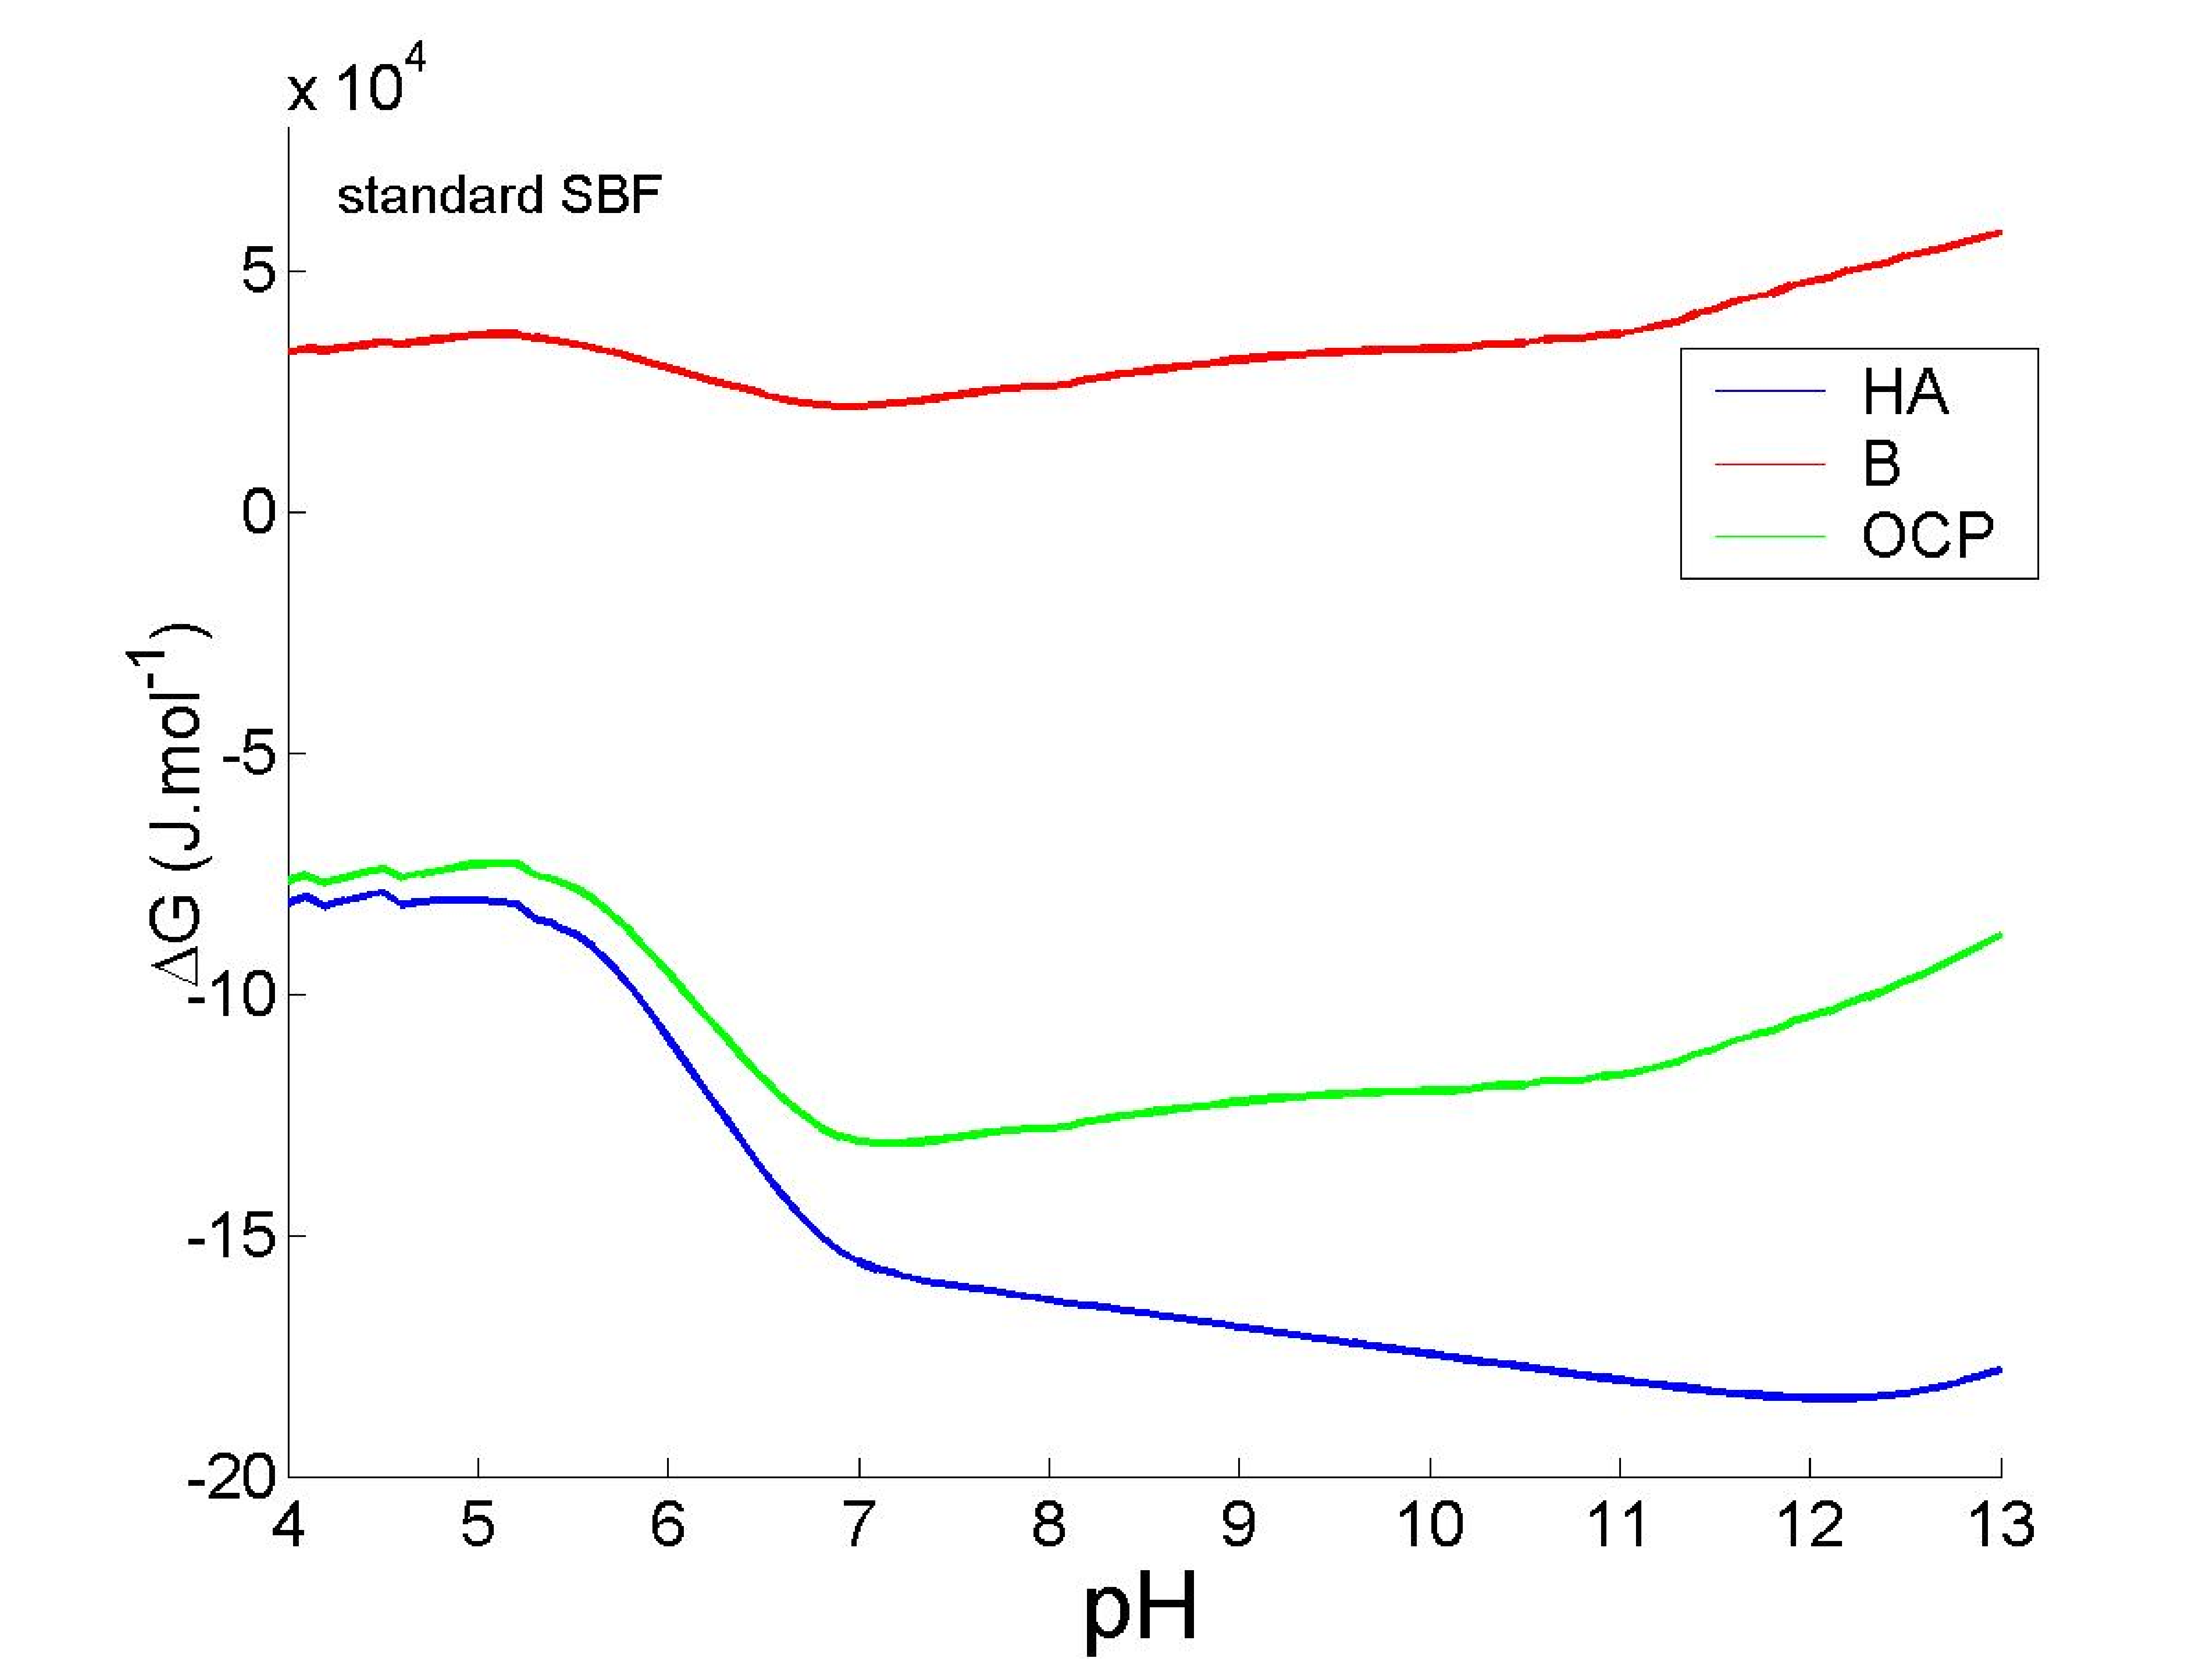
\includegraphics[height=6.7cm,width=9cm]{figura_1}%
\caption{Gibbs free energy variations: simulated results.}
\label{fig1}%
\end{center}
\end{figure}

Label coordinates in plots and add the corresponding units. Similarly, label
columns/rows in tables and add the units.

\subsection{Permission}
You are responsible for making sure that you have the right to publish
everything in your paper. If you use material from a copyrighted source, you
may need to obtain permission from the copyright holder.

\section{CALL TO REFERENCES IN THE BODY OF TEXT}
References should be cited in the text by name last (year) or (last name,
year). For example: ``In a recent work, Jones et al. (2005) proposed ...,'' or
``In a recent work (Devlou \& Zaparolli, 2013), it is suggested ... .''

References must be listed in alphabetical order at the end of the paper. Type
the word \textbf{REFERENCES} in all capitals, boldface type from the left
margin, skip one line and type the reference list. In each reference, indent
all lines 0.75 cm except the first line, which starts directly at the left
margin. Each reference must be cited in the text. In the section REFERENCES is
presented an example of a reference list including a journal article, a report,
an edited book, proceedings, a dissertation and a book.

\section{CONCLUSIONS}
This section should be included and need to show the main contributions of the
paper in a briefly form.

\subsection*{\textit{Acknowledgements}}
This section should be positioned between the end of the text and the reference
list. Type \textbf{\textit{Acknowledgements}} in boldface italics, skip one
line of space and type the text in regular type.


% ------------------------------------------------------------------------
\begin{thebibliography}{99}
\fontsize{11}{0}\selectfont
\bibitem[Aznar \& Pessoa, 1994]{Aznar94}
Aznar, M., Pessoa, F.L.P. and Silva Telles, A. (1994), ``Vapor-Liquid
Equilibria of Mixed Solvent-Salt Systems using a MHV2 Model with the Wilson
Equation'', {\em X Congresso Brasileiro de Engenharia Química}, São Paulo, vol
1, 38-43.

\bibitem[Freitas et~al., 2008]{Freitas08}
de Freitas, G.C.S.; Peixoto, F.C.; Vianna Jr, A.S. (2008), Simulation of a
thermal battery using Phoenics. Journal of Power Sources, 179, 424-429.

\bibitem[Duarte, 1999]{Duarte99}
Duarte, C.S.A. (1999), {\em Equilíbrio Líquido-Líquido em Sistemas contendo
Polímero e Eletrólito: Água/ Polietileno-glicol/Fosfato}, Laboratório de
Equilíbrio de Fases, FEQ/UNICAMP, Campinas.

\bibitem[Fredenslund, 1993]{Fredenslund93}
Fredenslund A. e Sorensen, J.M. (1993), ``Group Contribution Estimation
Methods'', in {\em  Models for Thermodynamic and Phase Equilibria
Calculations}, S.I. Sandler (ed.), Marcel Dekker, Inc., New York.

\bibitem[Silva, 2005]{Silva2005}
Silva, L.F. (2005), ``{\em Predição de Pontos Críticos de Misturas
Termodinâmicas}'', Tese de Doutorado, IPRJ/UERJ, Nova Friburgo.

\bibitem[Krevelenm, 1990]{Krevelen90}
Van Krevelen, D.W. (1990),{\em ``Properties of Polymers. Their Correlation with
Chemical Structure, Their Numerical Estimation and Prediction from Additive
Group Contribuition}'', 3º ed., Elsevier, Amsterdam.
\end{thebibliography}
\vspace*{-0.1cm}
\section*{APPENDIX A}
This section, if necessary, must be included here.

\vspace{0.5cm} % Example spaces

For Papers written in Portuguese or Spanish a translation of title, abstract
and keywords into English must be provided after the Appendix using the same
format for title, abstract and keywords presented in the first page of the
template.
% ------------------------------------------------------------------------

%For papers written in Portuguese or Spanish.

%\begin{center}
%  TITLE IN ENGLISH
%\end{center}

%\def\abstractname{Abstract}%

%\begin{abstract}
%   Abstract in english
%\end{abstract}

%\keywords{\em{Keywords in english}}

\end{document}
